\documentclass[../main]{subfiles}

\begin{document}
\chapter{Constructing New Vector Bundles Out of Old}\label{ch:3}

This section will describe a number of basic constructions involving vector bundles.
\begin{enumerate}
\item[(a)] \defemph{Restricting a bundle to a subset of the base space.}
\newline
Let $\xi$ be a vector bundle with projection $\pi : \total\varrightarrow{} \B$ and let $\xoverline{\B}$ be a subset of $\B$. Setting $\xoverline{\total}=\pi\inv(\xoverline{\B})$, and letting
\[
\xoverline{\pi} : \xoverline{\total}\longrightarrow \xoverline{\B}
\]
be the restriction of $\pi$ to $\xoverline{\total}$, one obtains a new vector bundle which will be denoted by $\xi|_{\xoverline{\B}}$, and called the \defemphi{restriction} of $\xi$ to $\xoverline{\B}$. Each fiber $F_b(\xi|_{\xoverline{\B}})$ is equal to the corresponding fiber $F_b(\xi)$, and is to be given the same vector space structure.

As an example if $M$ is a smooth manifold\index{smooth manifold} and $U$ is an open subset of $M$, then the tangent bundle $\tangentbundle{U}$ is equal to $\tangentbundle{M}|_{U}$\index{tangent bundle $\tangentbundle{M}$}.

More generally one has the following construction.


\item[(b)] \defemph{Induced bundles}.
\newline
Let $\xi$ be as above and let $\B_1$ be an arbitrary topological space. Given any map $f : \B_1\to \B$ one can construct the \defemphi{induced bundle} $f^*\xi$ over $\B_1$. The total space $\total_1$ of $f^*\xi$ is the subset $\total_1 \subset \B_1 \times \total$ consisting of all pairs $(b, e)$ with 
\[
f(b)=\pi(e).
\]
The projection map $\pi_1 : \total_1\varrightarrow{} \B_1$ is defined by $\pi_1(b,e)=b$. Thus one has a commutative diagram
\[
\begin{tikzcd}
	\total_1 \arrow[r, "\hat{f}"] \arrow[d, "\pi_1", swap] &\total \arrow["\pi", d] \\
	\B_1 \arrow[r, "f"]   & \B          
\end{tikzcd}
\]
where $\hat{f}(b, e) = e$. The vector space structure in $\pi_1\inv(b)$ is defined by
\[
t_1 (b, e_1) + t_2 (b, e_2) = (b, t_1 e_1 + t_2 e_2).
\]
Thus $\hat{f}$ carries each vector space $F_b(f^*\xi)$ isomorphically onto the vector space $F_{f(b)}(\xi)$.\end{enumerate}
If $(U,h)$ is a local coordinate system for $\xi$, set $U_1 = f\inv(U)$ and define
\[
h_{1} : U_{1} \times \bR^{n} \varrightarrow{} \pi_{1}\inv(U_{1}),
\]
by $h_{1}(b, x)=(b, h(f(b), x))$. Then $(U_1, h_1)$ is clearly a local coordinate system for $f^*\xi$. This proves that $f^*\xi$ is locally trivial. (If $\xi$ happens to be trivial, it follows that $f^*\xi$ is trivial.)


\begin{remark} \label{rem:03.01}
If $\xi$ is a smooth vector bundle\index{smooth vector bundle}\index{vector bundle!\indexline smooth} and $f$ a smooth map, then it can be shown that $\total_1$ is a smooth submanifold of $\B_1 \times \total$, and hence that $f^*\xi$ is also a smooth vector bundle.
\end{remark}


The above commutative diagram suggests the following concept which a priori, is more general. Let $\xi$ and $\eta$ be vector bundles.


\begin{definition}\label{def:03.01}
A \defemphi{bundle map} from $\eta$ to $\xi$ is a continuous function
\[
g:\total(\eta)\longrightarrow \total(\xi),
\]
which carries each vector space $F_b(\eta)$ isomorphically onto one of the vector spaces $F_{b'}(\xi)$.
\end{definition}

Setting $\xoverline{g}(b) = b'$, it is clear that the resulting function
\[
\xoverline{g} : \B(\eta)\varrightarrow{} \B(\xi),
\]
is continuous.


\begin{lemma}\label{lem:03.01}
If $g : \total(\eta)\varrightarrow{} \total(\xi)$ is a bundle map, and if $\xoverline{g} : \B(\eta)\rightarrow \B(\xi)$  is the corresponding map of base spaces, then $\eta$ is isomorphic to the induced bundle $\xoverline{g}^*\xi$.\index{base space}
\end{lemma}


\begin{proof}
Define $h : \total(\eta) \varrightarrow{} \total(\xoverline{g}^*\xi)$ by
\[
h(e)=(\pi(e),g(e))
\]
where $\pi$ denotes the projection map of $\eta$. Since $h$ is continuous and maps each fiber $F_b(\eta)$ isomorphically onto the corresponding fiber $F_b(\xoverline{g}^*\xi)$, it follows from Lemma~\ref{lem:02.03} that $h$ is an isomorphism.
\end{proof}


\begin{enumerate}
    \item[(c)] \defemph{Cartesian products}
\end{enumerate}
Given two vector bundles $\xi_1$, $\xi_2$ Projection maps $\pi_i : \total_i \varrightarrow{} \B_i$, $i =1, 2$, the \defemphi{Cartesian product}  $\xi_1\times\xi_2$ is defined to be the bundle with projection map
\[
\pi_1 \times \pi_2 : \total_1 \times \total_2 \varrightarrow{} \B_1\times\B_2;
\]
where each fiber
\[
(\pi_{1} \times \pi_{2})\inv (b_{1}, b_{2}) = F_{b_{1}}(\xi_{1}) \times F_{b_{2}} (\xi_{2}),
\]
is given the obvious vector space structure. Clearly $\xi_1\times\xi_2$ is locally trivial.

As an example, if $M = M_1 \times M_2$ is a product of smooth manifolds, then the tangent bundle $\tangentbundle{M}$ is isomorphic to $\tangentbundle{M_1}\times \tangentbundle{M_2}$\index{tangent bundle $\tangentbundle{M}$}. (Compare \ref{prob:1-A}.)
\begin{enumerate}
    \item[(d)] \defemph{Whitney sums}
\end{enumerate}
Next consider two bundles $\xi_1$, $\xi_2$ over the same base space $\B$. Let
\[
\Delta : \B\varrightarrow{} \B\times\B
\]
denote the diagonal embedding. The bundle $\Delta^*(\xi_1\times\xi_2)$ over $\B$ is
called the \defemphi{Whitney sum} of $\xi_1$ and $\xi_2$; and will denoted by $\xi_1\oplus\xi_2$. Note that each fiber $F_b(\xi_1\oplus\xi_2)$ is canonically isomorphic to the direct sum $F_b(\xi_1)\oplus F_b(\xi_2)$.


\begin{definition}\label{def:03.02}
Consider two vector bundles $\xi$ and $\eta$ over the same base space $\B$ with $\total(\xi ) \subset \total(\eta)$; then $\xi$ is a \defemphi{sub-bundle} of $\eta$ (written $\xi\subset\eta$) if each fiber $F_b(\xi)$ is a sub-vector-space of the corresponding fiber $F_b(\eta)$.
\end{definition}


\begin{lemma}\label{lem:03.02}
Let $\xi_1$ and $\xi_2$ be sub-bundles of $\eta$ such that each vector space $F_b (\eta)$ is equal to the direct sum of the sub-spaces $F_b (\xi_1)$ and $F_b (\xi_2)$. Then $\eta$ is isomorphic to the Whitney sum $\xi_1\oplus\xi_2$.
\end{lemma}


\begin{proof}
Define $f : \total(\xi_1\oplus\xi_2) \varrightarrow{} \total(\eta)$ by $f(b,e_1,e_2) = e_1 + e_2$. It follows from Lemma~\ref{lem:02.03} that $f$ is an isomorphism.
\end{proof}


\begin{enumerate}
    \item[(e)] \defemph{Orthogonal complements}
\end{enumerate}
This suggests the following question. Given a sub-bundle $\xi\subset\eta$ does there exist a complementary sub-bundle so that $\eta$ splits as a Whitney sum? If $\eta$ is provided with a Euclidean metric\index{Euclidean metric} then such a complementary summand can be constructed as follows.\footnote{If the base space $\B$ is paracompact\index{paracompact}, then $\eta$ can always be given a Euclidean metric (\ref{prob-2-C}); hence a sub-bundle $\xi\subset\eta$ is always a Whitney summand. If $\B$ is not required to be paracompact, then counterexamples can be given.}

Let $F_b(\xi^\perp)$ denote the subspace of $F_b(\eta)$ consisting of all vectors $v$ such that $v \cdot w = 0$ for all $w \in F_b(\xi)$. Let $\total(\xi^\perp) \subset \total(\eta)$ denote the union of the $F_b(\xi^\perp)$.


\begin{definition}\label{def:03.03}
$\xi^\perp$ will be called the \defemph{orthogonal complement}\index{orthogonal complement $\xi^\perp$} of $\xi$ in $\eta$.
\end{definition} %i know in the original the definition was between theorem and proof, but i think it looks nicer like this


\begin{theorem}\label{thm:03.03}
	$\total(\xi^\perp)$ is the total space of a sub-bundle
	$\xi^\perp\subset\eta$. Furthermore $\eta$ is isomorphic to the Whitney sum $\xi\oplus\xi^\perp$.
\end{theorem}


\begin{proof}
Clearly each vector space $F_b(\eta)$ is the direct sum of the sub-spaces $F_b(\xi)$ and $F_b(\xi^\perp)$. Thus the only problem is to prove that $\xi^\perp$ satisfies the local triviality condition.

Given any point $b_0 \in \B$, let $U$ be a neighborhood of $b_0$ which is sufficiently small that both $\xi|_U$ and $\eta|_U$ are trivial. Let $s_1, \dots, s_m$ be normal orthogonal cross-sections of $\xi|_U$ and let $s_1 ', \dots, s_n '$ be normal orthogonal cross-sections of $\eta|_U$; where $m$ and $n$ are the respective fiber dimensions. (Compare lemma \ref{lem:02.04}.) Thus the $m\times n$ matrix 
\[
\begin{bmatrix}
s_i (b_0) \cdot s_j ' (b_0)
\end{bmatrix}
\]
has rank $m$. Renumbering the $s_j '$ if necessary, we may assume that the first $m$ columns are linearly independent.

Let $V\subset U$ be the open set consisting of all points $b$ for which the first $m$ columns of the matrix $\big[s_{i}(b) \cdot s_{j}^{\prime}(b)\big]$  are linearly independent. Then the $n$ cross-sections
\[
s_1, s_2, \dots, s_m, s'_{m+1},\dots,s'_n
\] 
of $\eta|_U$ are not linearly dependent at any point of $V$. (For a linear relation would imply that some non-zero linear combination of $s_1 (b),\dots, s_m (b)$ was also a linear combination of $s'_{m+1} (b),\dots,s'_n (b)$, hence orthogonal to $s'_1 (b),\dots, s'_m (b)$.) Applying the Gram-Schmidt\index{Gram-Schmidt process} process to this sequence of
cross-sections, we obtain normal orthogonal cross-sections $s_1, \dots s_m,$ $s_{m+1},\dots,s_n$ of $\eta|_V$.

Now a local coordinate system
\[
h : V \times \bR^{n-m}\varrightarrow{} \total(\xi^\perp),
\]
for $\xi^\perp$ is given by the formula
\[
h(b, x)=x_{1} s_{m+1}(b)+\cdots+x_{n-m} s_{n}(b).
\]
The identity
\[
h\inv (e)=
(\pi e,(e \cdot s_{m+1}(\pi e), \dots, e \cdot s_{n}(\pi e))),
\]
shows that $h$ is a homeomorphism, and completes the proof of Theorem~\ref{thm:03.03}.
\end{proof}


As an example, suppose that $M\subset N\subset \bR^A$ are smooth manifolds, and suppose that $N$ is provided with a Riemannian metric. Then the tangent bundle $\tangentbundle{M}$\index{tangent bundle $\tangentbundle{M}$} is a sub-bundle of the restriction $\tangentbundle{N}|_M$. In this case the orthogonal complement $\tangentbundle{M}^\perp \subset\tangentbundle{N}|_M$ is called the \defemphi{normal bundle} $\normalbundle{}$ of $M$
in $N$. Thus we have:


\begin{corollary} \label{cor:03.04} 
For any smooth submanifold\index{submanifold} $M$ of a smooth Riemannian manifold\index{Riemannian manifold} $N$ the normal bundle $\normalbundle{}$ is defined, and
\[
\tangentbundle{M}\oplus\nu \cong \tangentbundle{N}|_M.
\]
\end{corollary}


More generally a smooth map $f : M \varrightarrow{} N$ between smooth manifolds is called an \defemphi{immersion} if the Jacobian\index{Jacobian $\dd f_x$}
\[
\differential{f}{x} : \tangentspace{M}{x} \varrightarrow{} \tangentspace{N}{f(x)}
\]
maps the tangent space $\tangentspace{M}{x}$\index{tangent space $\tangentspace{M}{x}$} injectively (i.e. with kernel zero) for each $x \in M$. [It follows from the implicit function theorem that an immersion is locally an embedding of $M$ in $N$, but in the large there may be self-intersections. A typical immersion of the circle in the plane is illustrated in \ref{fig:figure4}.]

\begin{figure}[ht]
    \centering
    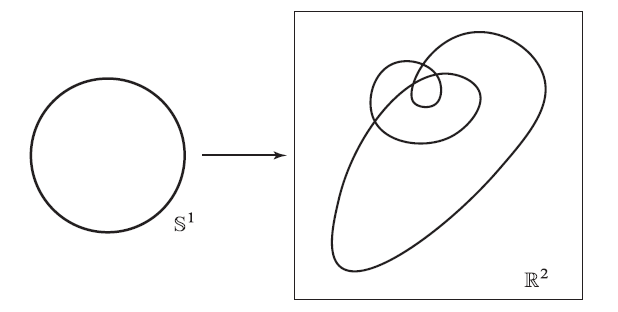
\includegraphics[scale=0.5]{"../tex from old group/fig4.png"}
    \caption{}
    \label{fig:figure4}
\end{figure}

Suppose that $N$ is a Riemannian manifold. Then for each $x\in M$, the
tangent space $\tangentspace{N}{f(x)}$ splits as the direct sum of the image $\differential{f}{x}(\tangentspace{M}{x})$ and its orthogonal complement. Correspondingly the induced bundle $f^* \tangentbundle{N}$ over $M$ splits as the Whitney sum of a sub-bundle isomorphic to $\tangentbundle{M}$ and a complementary sub-bundle $\normalbundle{f}$. Thus:


\begin{corollary}\label{cor:03.05}
For any immersion $f : M\varrightarrow{} N$, with $N$ Riemannian, there is a Whitney sum decomposition
\[
f^*\tangentbundle{N} \cong \tangentbundle{M} \oplus \normalbundle{f}.
\]
\end{corollary}
This bundle $\normalbundle{f}$ will be called the \defemph{normal bundle} of the immersion $f$.


\begin{enumerate}
    \item[(f)] \defemph{Continuous functors of vector spaces and vector bundles}
\end{enumerate}
The direct sum operation is perhaps the most important method for building new vector spaces out of old, but many other such constructions play an important role in differential geometry. For example, to any pair $V, W$ of real vector spaces\index{vector space} one can assign:

\begin{enumerate}\label{functors on vectors}
	\item[1)] the vector space $\Hom(V, W)$\index{Hom} of linear transformations from $V$ to  $W$;
	\item[2)] the tensor product\index{tensor product $\otimes$}\footnote{See for example \cite[pp. 408]{lang1965algebra}.} $V\otimes W$;
	\item[3)] the vector space of all symmetric bilinear\index{bilinear} transformations from $V \times V$ to $W$;
\end{enumerate}

and so on. To a single vector space $V$ one can assign:

\begin{enumerate} 
	\item[4)] the dual vector space\index{vector space!\indexline dual}\index{dual vector space} $\Hom(V, \bR) $; 
	\item[5)] the $k$-th exterior power\index{exterior power}\footnote{See for example \cite[pp. 424]{lang1965algebra}.} $\Lambda^k V$;
	\item[6)] the vector space of all $4$-linear transformations
	$V \times V\times V \times V\to \mathbb{R}$ satisfying the symmetry relations:
	\[
	K(v_1,v_2,v_3,v_4)=K(v_3,v_4,v_1,v_2)=-K(v_1,v_2,v_4,v_3)
	\]
	and
	\[
	K(v_1,v_2,v_3,v_4)+K(v_1,v_4,v_2,v_3)+K(v_1,v_3,v_4,v_2)=0.
	\]
\end{enumerate}

(This last example would be rather far-fetched, were it not important in the theory of Riemannian curvature\index{curvature}.)

These examples suggest that we consider a general functor of several vector space variables.


\begin{definition}\label{def:03.04}
Let $\vectCat_{\mathbb{R}}$ denote the category\index{category} consisting of all finite dimensional real
vector spaces and all isomorphisms between such vector spaces. By a
(covariant)\footnote{The distinction between covariant and contravariant functors is not important here, since we are working only with isomorphisms.} \defemphi{functor} $T : \vectCat_{\mathbb{R}}\times\vectCat_{\mathbb{R}} \varrightarrow{} \vectCat_{\mathbb{R}}$ is meant an operation which assigns
\begin{enumerate}
	\item to each pair $V, W\in \vectCat_{\mathbb{R}}$ of vector spaces a vector space $T(V, W)\in\vectCat_{\mathbb{R}}$;

and

	\item to each pair $f : V \to V'$, $g : W \to W'$ of isomorphisms an isomorphism
	\[
	T(f, g): T(V, W) \varrightarrow{} T(V', W');
	\]

so that

	\item $T(\id_V,\id_W)=\id_{T(V,W)}$ and
	\item $T(f_{1} \circ f_{2}, g_{1} \circ g_{2})=T(f_{1}, g_{1}) \circ T(f_{2}, g_{2})$.
\end{enumerate}
Such a functor will be called \defemph{continuous}\index{functor!\indexline continuous} if $T(f, g)$ depends continuously on $f$ and $g$. This makes sense, since the set of all isomorphisms from one finite dimensional vector space to another has a natural topology.
\end{definition}


The concept of a continuous functor $T : \vectCat_{\mathbb{R}}\times\dots\times\vectCat_{\mathbb{R}}\varrightarrow{}\vectCat_{\mathbb{R}}$ in $k$ variables is defined similarly. Note that examples 1, 2, 3 above are continuous functors of two variables, and that examples 4, 5, 6 are continuous functors of one variable.

Let $T:\vectCat_{\mathbb{R}}\times\dots\times\vectCat_{\mathbb{R}}\varrightarrow{}\vectCat_{\mathbb{R}}$ be such a continuous functor of $k$ variables, and let $\xi_1,\dots,\xi_k$ be vector bundles over a common base space $\B$. Then a new vector bundle over $\B$ is constructed as follows. For each $b\in \B$ let
\[
F_{b}=T(F_{b}(\xi_{1}), \dots, F_{b}(\xi_{k})).
\]
Let $\total$ denote the disjoint union of the vector spaces $F_b$ and define
$\pi:\total \varrightarrow{} B$ by $\pi(F_b) = b$.


\begin{theorem}\label{thm:03.06}
There exists a canonical topology for $\total$ so that $\total$ is the total space of a vector bundle with projection $\pi$ and with fibers $F_b$.
\end{theorem}


\begin{definition}\label{def:03.05}
This bundle will be denoted by $T(\xi_1,\dots,\xi_k)$.
\end{definition}


For example starting with the tensor product functor, this construction defines the \defemph{tensor product}\index{tensor product $\otimes$} $\xi\otimes\eta$ of two vector bundles. Starting with the direct sum functor one obtains the Whitney sum $\xi\oplus\eta$ of two bundles.
Starting with the duality functor
\[
V \mapsto \Hom(V,\bR),
\]
one obtains the functor
\[
\xi \mapsto \Hom(\xi,\trivialbundle^1),
\]
which assigns to each vector bundle its \defemph{dual vector bundle}\index{dual bundle}\index{vector bundle!\indexline dual}.

The proof of Theorem~\ref{thm:03.06} will be indicated only briefly. Let $(U,h_1),\dots, (U,h_k)$ be local coordinate systems for $(\xi_1,\dots,\xi_k)$ respectively, all using the same open set $U$. For each $b\in U$ define
\[
h_{ib}: \bR^{n_{i}} \longrightarrow F_{b}(\xi_{i}),
\]
by $h_{ib}(x)=h_i(b,x)$. Then the isomorphism
\[
T(h_{1 b}, \dots, h_{k b}): T(\mathbb{R}^{n_{1}}, \dots, \bR^{n_{k}}) \varrightarrow{} F_{b}
\]
is defined. The correspondence
\[
(b, x) \varrightarrow{} T(h_{1 b}, \dots, h_{k b})(x)
\]
defines a one-to-one function
\[
h: U \times T(\bR^{n_{1}}, \dots, \bR^{n_{k}}) \varrightarrow{} \pi\inv(U).
\]


\begin{assertion*}
There is a unique topology on $\total$ so that each such $h$ is a homeomorphism, and so that each $\pi^{-1}(U)$ is an open subset of $\total$.
\end{assertion*}


\begin{proof}
The uniqueness is clear. To prove existence, it is only
necessary to observe that if two such ``coordinate systems'' $(U,h)$ and $(U', h')$ overlap, then the transformation 
\[
(U \cap U') \times T(\bR^{n_1}, \dots, \bR^{n_k}) \varrightarrow{h\inv  h'} (U \cap U') \times T(\bR^{n_1}, \dots, \bR^{n_k})
\]
is continuous. This follows from the continuity of $T$.

It is now clear that $\pi: \total \varrightarrow{} \B$ is continuous, and that the resulting
vector bundle $T(\xi_1,\dots,\xi_k)$ satisfies the local triviality condition.
\end{proof}

\setcounter{remark}{0}
\begin{remark}\label{rem:03.02}
This construction can be translated into Steenrod's terminology as follows. Let $\GL_n = \GL_n(\bR)$\index{linear group $\GL_n$!\indexline real} denote the group of automorphisms of the vector space $\bR^n$. Then $T$ determines a continuous homomorphism from the product group $\GL_{n_1}\times\dots\times\GL_{n_k}$, to the group $\GL'$ of automorphisms of the vector space $T(\bR^{n_{1}}, \dots, \bR^{n_{k}})$. Hence given bundles $(\xi_1,\dots,\xi_k)$ over $\B$ with structural groups\index{structural group} $\GL_{n_1}\times\dots\times\GL_{n_k}$ respectively, there corresponds a bundle $T(\xi_1,\dots,\xi_k)$ with structural group $\GL'$ and with fiber $T(\bR^{n_{1}}, \dots, \bR^{n_{k}})$. For further discussion, see \cite[$\S$3.6]{hirzebruchalggeo1966}.
\end{remark}


\begin{remark}\label{rem:03.03}
Given bundles $(\xi_1,\dots,\xi_k)$ over distinct base spaces, a similar construction gives rise to a vector bundle $\xhat{T}(\xi_1,\dots,\xi_k)$ over $\B(\xi_1)\times\dots\times\B(\xi_k)$, with typical fiber $T(F_{b_1}(\xi_1)\times\dots\times F_{b_1}(\xi_k))$. This yields a functor $\xhat{T}$ from the category\index{category} of vector bundles and bundle maps into itself. As an example, starting from the direct sum functor $\oplus$ on the category $\vectCat_{\mathbb{R}}$ one obtains the Cartesian product functor\index{Cartesian product}
\[
\xi, \eta \mapsto \xi \xhat{\oplus} \eta=\xi \times \eta,
\]
for vector bundles.
\end{remark}


\begin{remark}\label{rem:03.04}
If $(\xi_1,\dots,\xi_k)$ are smooth vector bundles\index{vector bundle!\indexline smooth}\index{smooth vector bundle}, then $T(\xi_1,\dots,\xi_k)$ can also be given the structure of a smooth vector bundle. The proof is similar to that of Theorem~\ref{thm:03.06}. It is necessary to make use of the fact that the isomorphism $T(f_1,\dots,f_k)$ is a smooth function of the isomorphisms $T(f_1,\dots,f_k)$.
This follows from \cite[p. 128]{chevalley1999}.
\end{remark}


As an illustration, let $M \varrightarrow{f} N$ be a smooth map\index{smooth function}. Then $\Hom(\tangentbundle{M},f^*\tangentbundle{N})$ is a smooth vector bundle over $M$. Note that $\differential{f}{}$\index{derivative} gives rise to a smooth cross-section of this vector bundle.

As a second illustration, if $M\subset N$ with normal bundle $\normalbundle{}$, where $N$ is a smooth Riemannian manifold, then the \defemphi{second fundamental form} can be defined as a smooth symmetric cross-section of the bundle $\Hom(\tangentbundle{M}\otimes\tangentbundle{N}, \normalbundle{})$.
(Compare \cite{bishop2011}, as well as \ref{prob-5-B}.)

Here are six problems for the reader.

\begin{problem}\label{prob-3-A}
A smooth map $f : M \varrightarrow{}N$ between smooth manifolds is called a \defemphi{submersion} if each Jacobian
\[\differential{f}{x} : \tangentspace{M}{x} \varrightarrow{} \tangentspace{N}{f(x)}
\]
is surjective (i.e. is onto). Construct a vector bundle $\kappa_f$ built up out of the kernels of the $\differential{f}{x}$. If $M$ is Riemannian\index{Riemannian manifold}, show that
\[
\tangentbundle{M} \cong \kappa_f\oplus f^*\tangentbundle N.
\]
\end{problem}

\begin{problem}\label{prob-3-B}
Given vector bundles $\xi\subset\eta$ define the \defemphi{quotient bundle} $\eta/\xi$ and prove that it is locally trivial. If $\eta$ has a Euclidean metric,\index{orthogonal complement $\xi^\perp$}
show that

\[
\xi^\perp\cong\eta/\xi.
\]

\end{problem}
\begin{problem}\label{prob-3-C}
More generally let $\xi, \eta$ be arbitrary vector bundles over $\B$ and let $f$ be a cross-section of the bundle $\Hom(\xi, \eta)$\index{Hom}. If the rank of the linear function
\[
f(b) : F_b(\xi) \varrightarrow{} F_b(\eta)
\]
is locally constant as a function of $b$, define the kernel $\kappa_f\subset\xi$ and the cokernel $\normalbundle{f}$, and prove that they are locally trivial.
\end{problem}


\begin{problem}\label{prob-3-D}
If a vector bundle $\xi$ possesses a Euclidean metric,\index{Euclidean metric}
show that $\xi$ is isomorphic\index{isomorphic (vector bundles)} to its dual bundle $\Hom(\xi, \trivialbundle^1)$.\index{dual bundle}\index{vector bundle!\indexline dual}
\end{problem}


\begin{problem}\label{prob-3-E}
Show that the set of isomorphism classes of $1$-dimensional vector bundles over $\B$ forms an abelian group with respect to the tensor product operation. Show that a given $\bR^1$-bundle $\xi$ possesses a Euclidean metric if and only if $\xi$ represents an element of order $\leq 2$
in this group.
\end{problem}


\begin{problem}\label{prob-3-F}
(Compare \cite{Swan1962VectorBA}.) Let $\B$ be a Tychonoff space\footnote{A topological space is \defemph{Tychonoff} if it is Hausdorff, and if for every point $x$ and disjoint closed subset $A$ there exists a continuous real valued function separating $x$ from $A$. (Compare \cite{kelley1955}.)} and let $\mathbb{R}(\B)$ denote the ring of continuous real valued functions on $\B$. For any vector bundle $\xi$ over $\B$, let $S(\xi)$ denote the $\mathbb{R}(\B)$-module consisting of all cross-sections\index{cross-section} of $\xi$.
\begin{enumerate}
    \item Show that $S(\xi\oplus\eta)\cong S(\xi)\oplus S(\eta)$. Show that $\xi$ is trivial if and only if $S(\xi)$ is free.
	\item If $\xi\oplus\eta$ is trivial, show that $S(\xi)$ is a finitely generated projective module.\footnote{A module is \defemph{projective}\index{projective module} if it is a direct summand of a free module. See for example \cite[p. 368]{maclane1999algebra}.} Conversely if $Q$ is a finitely generated projective module
	over $\mathbb{R}(\B)$, show that $Q\cong S(\xi)$ for some $\xi$.
	\item Show that $\xi\cong\eta$ if and only if $S(\xi)\cong S(\eta)$.
\end{enumerate}
\end{problem}
\end{document}